\documentclass{article} % For LaTeX2e
\usepackage{nips15submit_e,times}
\usepackage{hyperref}
\usepackage{url}
\usepackage{graphicx}
\usepackage{subfig}
%\documentstyle[nips14submit_09,times,art10]{article} % For LaTeX 2.09


\title{Playing Go with Deep Learning}


\author{
Siddarth Sampangi \\
\And
Haresh Chudgar \\
\AND
Aditya Nagarajan \\
\And
Addison Mayberry \\
}

% The \author macro works with any number of authors. There are two commands
% used to separate the names and addresses of multiple authors: \And and \AND.
%
% Using \And between authors leaves it to \LaTeX{} to determine where to break
% the lines. Using \AND forces a linebreak at that point. So, if \LaTeX{}
% puts 3 of 4 authors names on the first line, and the last on the second
% line, try using \AND instead of \And before the third author name.

\newcommand{\fix}{\marginpar{FIX}}
\newcommand{\new}{\marginpar{NEW}}

\nipsfinalcopy % Uncomment for camera-ready version

\begin{document}


\maketitle

%!TEX root = nips2015.tex

\begin{abstract}
Our class project was to implement a DQN to play the game of Go, based on Nathan Sprague's Atari-playing agent. In this report we discuss the rules of Go and prior art in the field of Go-playing agents, and we describe our attempted implementation in terms of the techniques we tried and the problems we encountered. In the end, we were unable to get consistent results from our network due to a variety of extreme challenges inherent to this domain. We present an analysis of our results and other possible approaches that may better address the issues we encountered.
\end{abstract}

\section{The Game of Go}

Go is an ancient Chinese board game composed of a grid of intersecting perpendicular lines. The rules are simple - there are two players, and each player may place one piece (or ``stone'') on the board. Stones can only be placed on the intersection between two lines on the grid, and a player may only place a stone in a space that is not occupied by another stone. One player uses black stones, the other, white.

Go is widely considered to be the last largely unsolved classical game in the field of AI. This is due to two major contributing factors:

\begin{enumerate}
\item The extremely large possible number of games. A standard board has $19\times 19=361$ spaces in which to play, leading to $10^{171}$ possible board states - compare this to $10^{47}$ for chess. To consider all possible options for the next four moves would typically require examining $3.2\times 10^{11}$ possible board states.
\item The difficulty of evaluating a board state or evaluating the effectiveness of a given play. Go is known to be an extremely subtle game, with seemingly irrelevant plays in one area of the board having cascading effects only witnessed tens of moves later or more. This makes it extremely difficult for a machine to explore the space of potential moves or evaluate the current game state, even when guided by heuristics.
\end{enumerate}

Due to these limitations, no one has as of yet been able to successfully generate a Go agent that can compete at anything higher than a novice level. In this project, we attempted to expand upon (a) past work in the field of developing Go-playing agents and (b) recent work in developing deep-reinforcement-learning networks for playing games, in order to implement a deep-RL-based agent capable of playing Go at some level of competitiveness.

\section{Prior Art}
\label{gen_inst}

\subsection*{Monte Carlo Tree Search}
Prior to the recent successes in exploring the Go problem with machine learning techniques, the best results in the field of Go agents were obtained using Monte Carlo techniques. The best and most recent example of this technique was Baudis \& Gailly's Pachi [X], an open-source Go player built on the Monte Carlo Tree Search Algorithm (MCTS).

MCTS is based on an incrementally built probabilistic minimax tree. When the agent must make move, it takes the current game state as a node in the tree and expands out all possible moves this turn as child nodes. Any nodes already generated in previous iterations are included automatically. Whenever a new node is generated, it is assigned a score based on its expected value over the course of the game. This score is estimated by doing a series of Monte Carlo ``playouts,'' in which moves are chosen completely randomly or randomly with heuristics. There are a large variety of tunable parameters in this model - the number of MC playouts to compute, how and when to expand out all the children of a node explicitly, how to compute a node's score, and what heuristics (if any) to guide the MC player towards more likely or useful moves all must be chosen by the implementer.

Baudis \& Gailly iterated on a large body of MCTS-based Go work by adjusting the specific heuristics used for the MCTS player to include more advanced strategies. They do not present any quantitative measure of the strength of the Pachi player, but it was one of the first to play competitively against humans with some success. A side-by-side comparison of the following projects with Pachi included in [X] shows that it is weaker than the supervised learning approaches discussed next.

\subsection*{Deep Convolutional Neural Net}
There have been two major advances in developing Go agents with machine learning techniques in the past year. The first was Clark and Storkey's paper [X] which used a deep convolutional neural network (DCNN). The network was trained on two large publicly available datasets of Go games.

To compile the training data, the games were broken into individual moves. The input is the board state and the output is the move chosen by the player. The authors used a set of about 16.5 million board - move pairs between the two datasets.

The authors experimented with a number of board encoding techniques to attempt to explicitly inform the network about common abstractions that players of almost all levels use to make decisions about which move to play. The most basic input encoding they used had three channels - the first two to indicate the positions of stones of each player, and the third to enforce a simple rule that prevents the game from devolving into an infinite sequence of repeated plays - this rule is known as ``ko''. More advanced forms of board encodings they used explicitly captured simple features such as the the reflective properties of the game board or tactical information such as the number of ``liberties'' (neighboring empty board spaces) available to each piece on the board. They found that all of these encodings increased performance.

The best network architecture they reported involved eight layers. The first seven layers were convolutional layers with filters of decreasing size, which were zero-padded out to the width of the board to prevent the size of the outputs from progressively shrinking. The last layer was a fully-connected layer with a softmax output over the entire board, which is interpreted as the network's prediction of the most likely move a human player would make.

One game feature they were forced to encode directly into the DCNN was illegal moves, which ended up being a very difficult problem for us in our DQN implementation as discussed below. The basic rule of placement is simple - do not place a piece on top of another piece. However, as we discovered, teaching an agent not to do this directly from data can be extremely difficult. The authors attempted this by only backpropagating values on legal board positions during training and were able to teach the network to avoid most illegal moves, but still not all. In the end, they were forced to zero-out any output probability given to illegal moves during testing and re-normalize the remaining probability over the space of legal positions.

The results reported by these authors were, at time of publication, the best so far for any approach incorporating supervised learning. They reported a test accuracy of 44\% for predicting the move picked by a human player, and had a 91\% win rate against GnuGo, a popular open-source Go player. 

\subsection*{DCNN / Monte Carlo Hybrid}

Two very recent works, by Maddison et al. at DeepMind and by Tian \& Zhu at Facebook Research combined the described two techniques to yield the best results in the field so far [X]. They assert that one of the major weaknesses of the DCNN approach is its inability to search the space of moves, which makes it tactically weak as it cannot look ahead at the impact of future moves easily or naturally. They claim that search allows the agent to build a nonparametric local model based on the current state of the board, which has a great deal of utility alongside a global ``best-move'' model like the one provided by the DCNN implementation. Both the DeepMind and Facebook projects use MCTS to generate the search tree nodes, which are then passed to the DCNN component for evaluation. The two approaches differ in the method of synchronization - the DeepMind implementation allows the MCTS algorithm to run in parallel with the DCNN evaluation, whereas Facebook's system requires MCTS to halt until the DCNN evaluation of a node is completed. The former emphasizes high playout volume, the latter, better heuristic guidance of the rolled out nodes within MCTS. 

%!TEX root = nips2015.tex

\section{Deep Q Learning for solving Go}
In this section, we detail our initial motivation behind using the Deep Q Learning to solve Go. As detailed in the previous section, Go has been traditionally solved using Monte Carlo which searches through the complete state space of Go, however its time consuming considering the size of Go's state space. 
\\
A more elegant approach which is used by human experts is through finding shapes. Professional players analyse positions using a large vocabulary of shapes, such as joseki (corner patterns) and tesuji (tactical patterns). The most simple example is that of an atari which is shown in \textcolor{red}{Figure } to illustrate the idea. If we regard the game as an image, then a Convolution Neural Network can identify these patterns. This is probably the reason behind success of convolution neural network. However a CNN can only look through the next move and thus fares badly against a Monte Carlo which can evaluate multiple moves.
\\
\begin{figure}[h]
	\centering
	\subfloat[Example 1: The white stones are all in atari and can be captured if black plays the next move]{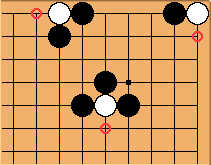
\includegraphics[width=0.47\textwidth]{atari_1}\label{fig:Gamma_0.7}}
	\hfill
	\subfloat[Example 2:The five black stones on the top right are in atari. The only liberty they have is the circled intersection.
	The group of two black stones on the lower left is also in atari. It may be captured by white (when white plays at a).]{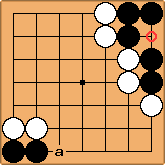
\includegraphics[width=0.43\textwidth]{atari_2}\label{fig:Karpathy}}
	\caption{Concept of Atari}
\end{figure}
\\
Our approach combines the benefit of visualizing shapes through CNN and looking ahead through Q Learning using a discount factor greater than 0. It is similar to the approach used by Facebook but it is more elegant as look ahead and shape recognition are combined in the same algorithm rather than being separate.

%!TEX root = nips2015.tex
\section{Initial Setup}

\subsection*{Building an Opposing Player}

Our first goal was to choose an enemy agent for the DQN to play against while learning. We evaluated three different enemies.

1. Clark \& Storkey's trained DCNN model: \\

Clark \& Storkey used ConnetJS to build their network. To use their network, we had to convert parse their network file and import it to lasagne. We found that the converted network was not playing as well as the online version posted by the authors. This is probably because ConvnetJS and Lasagne represent weights differently. Not to loose more time, we moved to evaluating other approaches.
\\
2. Pachi/Michi: 
\\
We next turned to Pachi, Baudis \& Gailly's MCTS-based player. While playing against it, we realized the speed  We were able to get it working, but it was very slow to compute the next move, taking almost a second or two. This would have been far too slow to be useful for the purpose of running hundreds of training epochs for the DQN.
\\
3. GnuGo:
\\
We finally settled on GnuGo, a standard open-source heuristic-based Go player. This program is the baseline for comparison in most of the recent papers on Go, so we considered it to be a good choice for training our agent. GnuGo has a scale of difficulty levels it will play at, from 1 to 10, with 10 being the most advanced. There is a tradeoff, however, as more advanced levels also take significantly more time to decide on a move. We left it at the default setting of 10 in order to push our agent towards better play from the beginning.

\subsection*{Porting the Atari Agent}

We based our work on Nathan Sprague's Atari-playing code from the midterm project. Fortunately, the interface between the learner and ALE was designed to abstract away most of the details specific to any particular Atari game, since they needed to be able to run it over all of the games in the list. We were able to swap out ALE for GnuGo by doing a few minor modifications to the training code and creating a simple interface from GnuGo to the DQN trainer. This allowed the training code to request score and game state from GnuGo the same as it did with ALE.

Another important change we had to make was the input representation. We wanted to try out different representations of the go game and evaluate each one of them. This part was a bit tricky as the input representation is tied with almost every class in the code.

%!TEX root = nips2015.tex
\section{Experiments}
There are three major parameters in our system:
\\
1. Input representation of the game:
\\
We evaluated three different matrix representations of the Go board.
\\
i. One channel representation: Translating the board to a matrix directly by encoding a white stone as 255, a black stone as 0 and an empty position as 127. This was nearest to the Atari representation.
\\ii. Three channel representation: The first and second channels encode black and white stones respectively by placing a one in the matrix if there is a stone, 0 otherwise. The third channel places a one if there is a stone, zero if it is empty; this is basically the sum of first two channels.
\\
iii. Seven channel representation: This is inspired from Clark \& Storkey's input to the CNN which encodes information about the game itself by using the concept of liberties. A stone is said to have four liberties if the position to its left and right, top and bottom are empty, three if one of these positions is occupied by a competing stone and so on. If two stones of the same color are adjacent the liberties of each stone increases [figure]. In this representation, we encode black positions in the first three channels by placing a one in the first channel if that stone has more than three liberties, one in the second channel if that stone has two, and one in the last channel if that stone has one liberty. The next three channels similarly encode positions of white stones. Each channel has a padding of three on either sides, so each channel of a 7 x 7 board will be of size 10 x 10. For the first six channels the padding is set to 0, whereas the seventh channel is 0 everywhere except at the padding where it is set to 1. This padding encodes the board's boundary.
\\
2. Architecture of the convolution neural network
\\
Briefly, the different network configurations we used are as follows:
\\
i. Two layer CNN with one dense layer and one softmax
\\
ii. Three layer CNN with one dense layer and one softmax
\\
iii. Five layer CNN with one dense layer
\\
iV. Seven layer CNN with one dense layer
\\
v. Five layer CNN with one dense layer and one multiplicative layer which zeroes out the q values of illegal moves
\\
In addition, we varied the filter sizes of the convolution layers.
\\
3. Parameters of Q Learning
\\
We varied the experience replay size and discount factor to find the right range of values. 
\\


%!TEX root = nips2015.tex
\section{Analysis and Future Work}
In this section, we offer hypotheses that attempt to explain why our agent was not able to learn an appropriate Q-network for Go. First, we simply could not generate a sufficient number of quality training examples. A large number of our training examples were illegal moves with a reward of -1. Even if we disregard this, the speed with which we were able to generate training examples was simply far from sufficient. Considering that [2] trained on 16 million examples, and that, assuming approximately 50 moves per game on a board of size 7, it took us 3 days to generate 100,000 examples, it is simply infeasible to expect to generate a data set of comparable size. We must then rely on using training examples in a more efficient way, or we must avoid training a network from scratch.

As mentioned before, weight tying is one way to use training examples more efficiently, and initializing the Q-network to a DCNN would definitely help with avoiding illegal moves. Still, weight tying only offers an improvement of an approximate factor of 8. We can think of this as allowing us to generate 800,000 moves in 3 days, which is still far from satisfactory. It might very well be completely necessary to use a combination approach involving Monte-Carlo and convolutional networks, as recent results indicate. 

While we have not been able to train a Q-network, we believe that we have still made a contribution to the community with our code. As of now, anyone can download our code from github and quickly experiment with their own modifications to the Q-network or other modules. Just as the open source ALE environment allowed DeepMind to test their system, our code will allow others in the community to test their strategies on Go.

We tested out different configurations of the experiments mentioned in the last section and evaluated them using the difference in scores of the network and GnuGo. We expected that, as the network improved its tactics, the changes would manifest in the GnuGo opponent having more difficulty scoring higher points thus increasing the difference from negative to positive.

Unfortunately, in all cases we were unable to get consistent performance, regardless of specific parameter settings. It did win occasionally, but overall GnuGo beat the network consistently. In the games which it won, we could not make out a clear strategy so we assume its a one off game. Figure \ref{fig:score} shows one particular training session that we allowed to run for 2000 games. 

\subsubsection*{References}

\small{
[1] Baudi�, Petr, and Jean-loup Gailly. "Pachi: State of the art open source Go program." {\it Advances in Computer Games. Springer Berlin Heidelberg}, 2012. 24-38.

[2] Clark, C. \& Storkey, A. (2015) Training Deep Convolutional Neural Networks to Play Go. {\it Proceedings of the 32nd International Conference on Machine Learning - ICML '15.}

[3] Maddison, C. J., Huang, A., Sutskever, I., \& Silver, D. Move Evaluation in Go Using Deep Convolutional Neural Networks. arXiv preprint arXiv:1412.6564. 2015.

[4] Tian, Y., \& Zhu, Y. (2015). Better Computer Go Player with Neural Network and Long-term Prediction. arXiv preprint arXiv:1511.06410. 2015.
}

\end{document}
